\documentclass[11pt]{article}

\usepackage[utf8]{inputenc}
\input{glyphtounicode}
\pdfgentounicode=1
\usepackage{amsmath,amssymb}
\usepackage{booktabs}
\usepackage{xcolor}
\usepackage{graphicx}
\usepackage{hyperref}
\usepackage[margin=1in]{geometry}
\usepackage{url}
\def\UrlBreaks{\do\/\do-\do_}

\hypersetup{colorlinks=true, linkcolor=blue, citecolor=blue, urlcolor=blue}
\setlength{\tabcolsep}{4pt}
% Open items of this draft are marked in red; none of them is a result.
\newcommand{\todo}[1]{\textcolor{red}{[TODO: #1]}}
\newcommand{\pending}{\textcolor{red}{\textbf{[DAY 3 PENDING]}}}
\newcommand{\checkref}{\textcolor{red}{\textbf{[CHECK]}}}
% Source convention: every number carries a comment "% src: results/..." (TOQB) or
% "% src: numbers.json ..." (readable_depth_self_check_numbers.json, written by
% readable_depth_self_check_figures.py from TOQB's raw counts).

\title{What Sets the Readable Depth of a Placed Ring, and How Far a Self-Checking Layer Pushes It:\\
Scan, Register, Avoid and Repair on Three Heavy-Hex Devices Without the Calibration Map}

\author{TN Holdings\\
\texttt{love.os.architect@proton.me}\\
\texttt{https://github.com/TN-Holdings-LLC/psf-zero}}

\date{Draft --- 2 November 2026 (workplace draft; numbers of 2 November pending)}

\begin{document}
\maketitle

\begin{abstract}
A circuit placed on a superconducting device stays readable only to some depth. In earlier work we measured that
depth without reading the calibration map and found, on \texttt{ibm\_kingston}, a stretch of a ring whose echo was
near random or inverted while the calibration showed nothing there. Here we ask what sets the readable depth on a
given day and device, and how much of it a user-side layer can recover from its own runs alone. The layer tests the
rings it would use with a mirror echo read per site, keeps a list of the paths it found dead (listed after two jobs,
expired after seven days), places the next ring around them with the same formula, and, only for mirror-type
circuits, applies a local frame flip that leaves the ideal circuit unchanged. All tests were declared before their
fetch, and the placement is fold:rule against fold:rule throughout. Two effects are kept apart. \emph{Width}: where a
dead run sat on the standard ring, avoiding it made every site usable again (kingston $n=40$: 22 of 40 to 40 of 40 on
two days; $n=72$: 38--39 to 72), and on two more devices the same scan-then-avoid widened the ring
(\texttt{ibm\_fez} $n=40$: 29 to 40, $n=72$: 36 to 63; \texttt{ibm\_marrakesh} $n=72$: 67 to 72). \emph{Accuracy}: on a
ring that was already fully usable, a forward Clifford computation with a known answer was slightly more right on the
avoiding ring (marrakesh, $n=72$: mean site signal 0.776 to 0.816 at 12 layers, 0.643 to 0.694 at 24), and all of the
gain sat in the ten qubits that the avoiding ring replaced. The ring avoiding the registry reached the depth of the
$n=20$ control at $n=40$ but not at $n=72$, where a shortfall of about two layers remained with no weak run visible to
the scan. A two-qubit frame flip lifted kingston's dead block by $+0.32$ and $+0.30$ on two days without cost
elsewhere, but recovered it only to about a third of the healthy sites at 24 layers. Avoiding comes first; repair is for
a ring that cannot avoid the path. A planned third day is pending.
\end{abstract}

\section{Introduction}

\begin{itemize}
\item \textbf{The question.} Paper~5 \cite{paper5} measured how deep a ring stays readable on IBM's heavy-hex devices
  when no placement reads a quality number, as the decay length $L^*$, and reported a defect that no calibration
  number shows. Here we ask two things: (i) what sets that depth on a given day and device, and (ii) how much of it a
  layer on the user's side can recover using only its own runs.
\item \textbf{An analogy, for the reader only.} An operating system tests its memory (memtest), keeps a list of bad
  blocks, allocates around them, and sometimes patches around a fault. The layer here does the same with a mirror echo,
  a list of dead paths, the ring placement and a frame flip. Like Paper~5's acoustic picture, this is an analogy, not
  an identity.
\item \textbf{Two effects, kept apart from the start.} \emph{Width}: how many ring sites still carry information
  (usable sites). \emph{Accuracy}: how right the output is on a ring that is already fully usable. The same ``$+x$'' can
  mean either; every result in Section~\ref{sec:results} says which one it is.
\item \textbf{What is new.} (1) A self-measured defect registry that holds paths, not qubits, with dates and expiry,
  built from the user's own jobs and no quality number. (2) Declared tests of scan, then avoid, on three devices. (3)
  The separation of width and accuracy gains, including a forward computation. (4) Repair by a local frame flip, with
  its limits.
\item \textbf{What is not new.} Mirror circuits as benchmarks \cite{proctor2022}; layer fidelity and errors per layered
  gate \cite{mckay2023}; noise-aware layout from calibration data (for example Qiskit's VF2 post-layout pass, which
  scores layouts with the target's error rates \cite{vf2post}); fluctuations of qubit quality in time from two-level
  defects \cite{klimov2018}; Pauli-frame and twirling identities \cite{wallman2016}. The placement formula and its
  comparison with other placements are Paper~4 \cite{paper4} and Paper~5 \cite{paper5}; they are not repeated here.
\end{itemize}

\section{Yardsticks}\label{sec:yardsticks}

Five quantities appear below. They answer different questions, and their numbers are never put side by side as
``deeper'' or ``shallower''. Ratios are taken only within one row (standard against avoiding ring, same device and
day).

\begin{table}[h]
\centering\footnotesize
\begin{tabular}{p{2.3cm}p{4.3cm}p{2.4cm}p{1.4cm}p{3.6cm}}
\toprule
& what is read & depth unit & records & typical rule values \\
\midrule
Y1 charge $L^*$ & four-input ratio of the weight-2 charge & one-way steps $L$ & 29 Oct & kingston 81--90, marrakesh 56--57 \\
Y2 echo $L^*$ & four-input ratio $\rho_E$ of the mirror echo & echo layers $D$ (both ways) & 30 Oct on & kingston 22--26 ($n=20$, 36) \\
Y3 site signal & per-site echo signal $a_j$ at $D=24$ & --- & 30 Oct on & healthy 0.35--0.45 \\
Y4 forward signal & per-site signal of an identity Clifford circuit & layers $D$ & 1 Nov & marrakesh $n=72$: 0.78--0.82 ($D=12$) \\
Y5 parity $V^*$ & weight-$n$ parity, fitted on $nL$ & $nL$ & 30 Oct & kingston 73--106 \\
\bottomrule
\end{tabular}
% src: Y1 results/noise-wall-1-kingston-2026-10-29/README.md, results/noise-wall-1-marrakesh-2026-10-29/README.md (rule only; Paper 5)
% src: Y2 results/device-2026-10-31-fez/README.md ("kingston 22-26 steps at n = 20, 36"), results/device-2026-10-30/
% src: Y3 results/clean-depth-2026-10-31/README.md (n = 20, 40: 0.35 or more), results/safe-ladder-2026-10-31/README.md (medians 0.39-0.45)
% src: Y4 results/qca-m3b-2026-11-01/score_V.json, score_S.json (means 0.776 / 0.816 at D = 12)
% src: Y5 results/device-2026-10-30/README.md (test 3P: V*_rule kingston 72.6, 105.8)
\caption{The yardsticks. Y1 and Y2 differ both in the observable (a conserved weight-2 charge against a local echo
that spreads) and in the unit (one-way steps against both-way layers).}
\label{tab:yard}
\end{table}

\begin{itemize}
\item \textbf{Site classes (Y3).} A site is \emph{dead} if $a_j<0.12$; a dead run is at least three consecutive dead
  ring sites (cyclic). A site is \emph{weak} if $a_j<\max(0.12,\ 0.5\times\text{ring median})$; a weak run likewise.
  The \emph{usable} sites are those outside every dead run. These rules were written before the coverage-days
  declaration (TOQB \texttt{toqb/defect\_list.py}, \texttt{toqb/safe\_loop.py}) and are used unchanged.
\item \textbf{Registry entry.} The four qubits at the centre of a dead run (a \emph{path}). Two sightings sharing two
  qubits are the same defect. A path is LISTED after two jobs and EXPIRED seven days after it was last seen.
\end{itemize}

\section{What sets the readable depth}\label{sec:what}

\subsection{The placement}
Held fixed here (the rule). Its advantage over the other map-free placements, in $\Delta L$ and in 0 losses of 144
echo comparisons, is Paper~5's result \cite{paper5}.

\subsection{The observable}
\begin{itemize}
\item The charge is conserved by the circuit and stays a weight-2 quantity; its $L^*$ (Y1) is long.
\item The echo's local $Z_j$ spreads within the light cone of the circuit; its $L^*$ (Y2) is shorter, but at $D=24$ the
  rule's $\rho_E$ did not shrink with $n$ up to 72 (0.17--0.44 across devices and sizes).
  % src: results/device-2026-10-30/README.md ("0.17-0.44 at D = 24 and does not shrink with n up to 72")
\item The parity has weight $n$; at $n\ge40$ its readout reference itself fell towards zero, so the parity's size wall
  on these devices was set by readout.
  % src: results/device-2026-10-30/README.md (test 3P: reference 0.4-0.6 at n = 20, 0.1-0.3 at n = 40, about 0 on marrakesh at n = 72)
\item \textbf{A failed prediction.} A trajectory twin with $T_1$, $T_2$ and static $ZZ$ predicted the echo at
  0.08--0.10 for $n=20$, $D=24$, and below the noise floor at $n=40$ and 72. The device gave 0.17--0.44.
  % src: results/pod-2026-10-30/ (twin rho_E 0.0844-0.0994), results/device-2026-10-30/README.md ("Failed prediction")
\end{itemize}

\subsection{Defects on the ring}
\begin{itemize}
\item \textbf{Black.} The same 18 qubits (3--7, 17, 27--29, 38, 49--55, 59) formed a dead run on the standard $n=40$
  ring of \texttt{ibm\_kingston} in every run of the byte-identical circuit: on 30 October, 31 October and 1 November
  (Figure~\ref{fig:sites}). Seventeen of these 18 qubits were healthy on other rings the same day, so the defect
  belongs to a path, not to the qubits.
  % src: numbers.json fig1 (dead runs of the three days); results/defect-list-replay-2026-10-31/README.md (17 of 18 healthy elsewhere)
\item \textbf{Gray.} A weak stretch (35, 19, 15, 14) on an $n=72$ ring read 0.10--0.12 at 11:40 CET and 0.46--0.49 at
  13:14 CET on 31 October, with the same circuit on the same qubits.
  % src: results/gray-stage1-2026-10-31/README.md, gray_score.json
\item \textbf{A coherent part.} Dynamical decoupling did not lift the dead sites, and gate twirling turned their
  inversion into noise; the block's signal crossed zero over depth (between $D=16$ and $D=20$); a frame flip brought
  part of it back (Section~\ref{sec:repair}).
  % src: results/device-2026-10-30/options-test/README.md (G -0.133 off, -0.115 dd, 0.010 twirl); results/black-stage1-2026-10-31/README.md (J1 CROSSES ONCE)
\item \textbf{Chip, and partly position.} The byte-identical $n=20$ circuit had no dead run on kingston and lost 11 of
  20 sites on \texttt{ibm\_fez}. On the other hand, some ring positions (positions 57--64 of the $n=72$ ring) were weak
  on all three chips. The defects depend on the chip, and some positions repeat across chips.
  % src: results/device-2026-10-31-fez/README.md (11 of 20); results/defect-list-replay-2026-10-31/README.md (positions 57-64)
\end{itemize}

\subsection{A size effect with no visible defect}
On rings with no weak run at all, the rings of $n=48$--72 read about two layers shallower than the $n=20$ control of
the same job (Y2 $L^*$ 21.3--22.3 against 24.1), and the $n=72$ ring placed around the registry was SHORTER by the
clean-depth test (20.4--20.8 against 23.9--24.7). We do not know why; it is reported as open.
% src: results/safe-ladder-2026-10-31/README.md (round 1: 22.26, 22.31, 21.30, 22.02 against 24.07); results/clean-depth-2026-10-31/judgement.json

\section{The self-checking layer}\label{sec:layer}

\begin{table}[h]
\centering\small
\resizebox{\textwidth}{!}{\begin{tabular}{lll}
\toprule
layer & function & records \\
\midrule
L1 scan & mirror echo per site on the rule's standard rings ($n=20,40,72$; $D=24$) & coverage days, two devices \\
L2 registry & black paths (LISTED after 2 jobs, 7-day expiry); gray paths for the day only & \texttt{list\_after.json} files \\
L3 allocate & the rule's placement with the middle coupler of each listed path marked failed & coverage B, clean depth, M3 \\
L4 repair & local frame flip, mirror-type circuits only, entries verified on two days & black stages 2--3, fix, fix repeat \\
\bottomrule
\end{tabular}}
\caption{The layers used in the declared tests. A sentinel layer (echo circuits riding in the user's job) is planned
and not yet tested.}
\label{tab:layers}
\end{table}

\begin{itemize}
\item \textbf{Map-free.} No calibration quality number is read; only the coupling graph, the basis and the failed
  elements.
\item \textbf{Self-measured.} Every registry entry comes from the user's own runs, with dates.
\item \textbf{Avoid by default.} Repair only with an entry verified on two days, and only for mirror circuits.
\item \textbf{Black carried, gray not.} Black entries carry over days; gray ones apply on the day they were seen.
\item \textbf{No cause chased.} An entry is kept or dropped by what it does.
\item \textbf{Declared.} Each claim is a declared test (Table~\ref{tab:decl}), with stop rules that weigh the size of
  effects (Section~\ref{sec:failures}).
\item \textbf{Cost.} A scan is 24 circuits; it was billed 9 s per device, and is skipped when the registry already
  holds a scan of the day.
  % src: results/coverage-days-2026-10-31-day1/README.md (job A, 24 circuits, 9 s billed); results/two-devices-2026-11-01/README.md (scan jobs 9 s)
\end{itemize}

\section{Results}\label{sec:results}

\subsection{Width: usable sites (Y3)}\label{sec:width}

\begin{table}[h]
\centering\small
\resizebox{\textwidth}{!}{\begin{tabular}{lccl}
\toprule
device, day & $n=40$: standard $\to$ avoiding & $n=72$: standard $\to$ avoiding & verdicts \\
\midrule
kingston, 31 Oct (coverage day 1) & 22 $\to$ 40 & 38 $\to$ 72 & WIDER, WIDER \\
kingston, 1 Nov (coverage day 2) & 22 $\to$ 40 & 39 $\to$ 72 & WIDER, WIDER \\
fez, 1 Nov & 29 $\to$ 40 & 36 $\to$ 63 & HELPS \\
marrakesh, 1 Nov & 40 $\to$ 40 & 67 $\to$ 72 & HELPS \\
kingston, 2 Nov (coverage day 3) & \pending & \pending & \pending \\
\bottomrule
\end{tabular}}
% src: numbers.json width (from results/coverage-days-2026-10-31-day1/coverage.json, results/coverage-days-2026-11-01-day2/coverage.json,
% src:   results/two-devices-2026-11-01/fez/avoid/coverage.json, results/two-devices-2026-11-01/marrakesh/avoid/coverage.json)
% src: verdicts: results/coverage-days-2026-11-01-day2/README.md, results/two-devices-2026-11-01/README.md
\caption{Usable sites on the standard ring and on the ring placed around the registry, same device and day.}
\label{tab:width}
\end{table}

\begin{figure}[h]
\centering
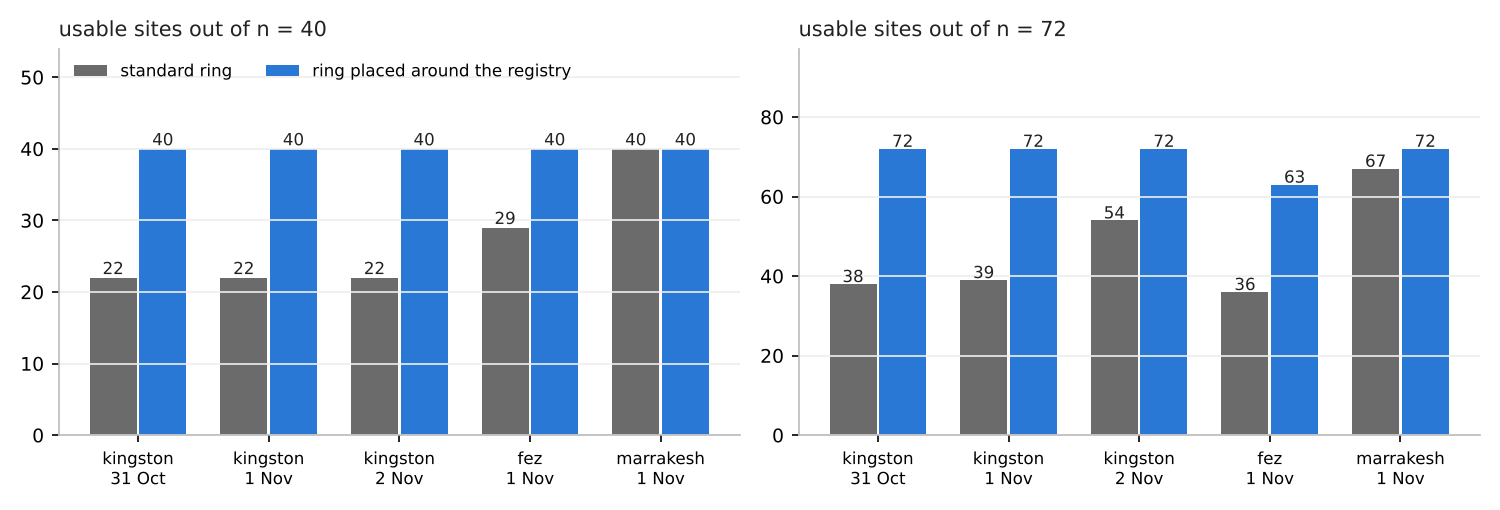
\includegraphics[width=\textwidth]{figures/self_check_width.png}
\caption{Usable sites, standard ring (grey) against the ring placed around the registry (blue). From the coverage
files of each test.}
\label{fig:width}
\end{figure}

\begin{figure}[h]
\centering
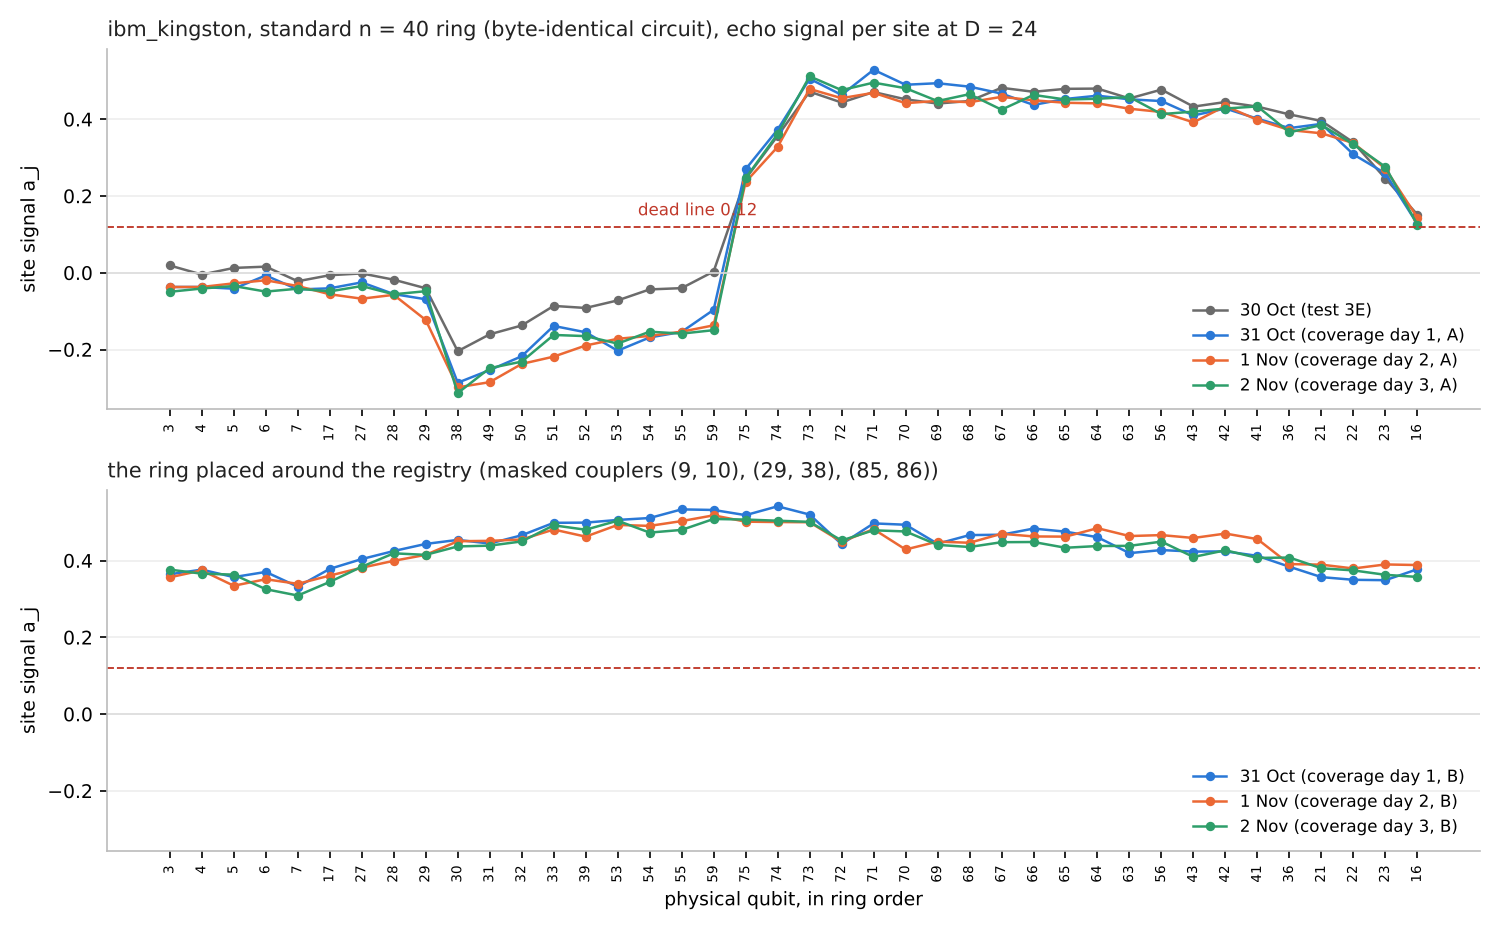
\includegraphics[width=\textwidth]{figures/self_check_kingston_n40_sites.png}
\caption{Top: the per-site echo signal along kingston's standard $n=40$ ring on three days (byte-identical circuit).
The run 3--59 is below the dead line every time. Bottom: the ring placed around the registry, same days.}
\label{fig:sites}
\end{figure}

\begin{itemize}
\item \textbf{The show-off number and the essential one.} The show-off number is usable sites 22 $\to$ 40. The essential
  one: on the sites that were already usable, the mean signal moved only 0.41 $\to$ 0.44 (day 1) and 0.39 $\to$ 0.44
  (day 2). The gain is width. The whole-ring mean (0.17 $\to$ 0.44) mixes both effects and is not used as a headline.
  % src: numbers.json width "kingston 31 Oct n40" mean_usable (0.410, 0.441), mean_all (0.175, 0.441); "kingston 1 Nov n40" (0.393, 0.438)
\item \textbf{The defect stayed where it was.} On both days the listed path [28, 29, 38, 49] was dead on the standard
  ring (PRESENT), and the avoiding rings had no dead run.
  % src: results/coverage-days-2026-10-31-day1/README.md, results/coverage-days-2026-11-01-day2/README.md
\item \textbf{Not everything was masked.} On fez the avoiding $n=72$ ring still carried a nine-site dead run next to a
  listed path; it entered the registry for the next day.
  % src: results/two-devices-2026-11-01/README.md
\item \textbf{When there is nothing to avoid.} On marrakesh at $n=40$ the standard ring had no dead run, and the avoiding
  ring changed nothing (SAME).
\item \textbf{Day 3.} Whether the black entries persist over three days is \pending.
\end{itemize}

\subsection{Depth recovered (Y2, rings placed around the registry)}
\begin{table}[h]
\centering\small
\begin{tabular}{llll}
\toprule
ring & standard ring (30 Oct) & avoiding ring (31 Oct) & verdict against the $n=20$ control \\
\midrule
kingston $n=40$ & 13.0--16.0 & 24.2--24.6 & REACHED (3 of 3 $h_z$) \\
kingston $n=72$ & 14.6--16.0 & 20.4--20.8 & SHORTER (3 of 3 $h_z$) \\
\bottomrule
\end{tabular}
% src: results/clean-depth-2026-10-31/README.md and judgement.json (hz 0, 0.1, 0.3)
\caption{Echo $L^*$ (layers $D$, Y2) on kingston. The $n=20$ control read 23.9--24.7 in the same job.}
\label{tab:depth}
\end{table}

\begin{itemize}
\item \textbf{A stricter list does not close the gap at $n=72$.} With weak runs listed too (the safe ladder), the safe
  size of that day was $n=40$; $n=48$ to 72 had no weak run and were still about two layers short, so the scan cannot
  see what remains (Section~\ref{sec:what}).
  % src: results/safe-ladder-2026-10-31/README.md
\end{itemize}

\subsection{Accuracy: a forward computation on a fully usable ring (Y4)}\label{sec:accuracy}

\begin{itemize}
\item \textbf{Circuit.} $D$ layers alternating (S on all, CZ ring) and (H on all, CZ ring). It is the identity whenever
  $D$ is a multiple of 6, at every ring length, and it is not a mirror: no layer is undone by a later one. The answer
  is the input, bit by bit, on four inputs.
\item \textbf{Test.} \texttt{ibm\_marrakesh}, $n=72$, the standard ring (holding the listed coupler (27, 28)) against
  the ring placed around the registry. Both jobs ran within one second of each other.
  % src: results/qca-m3b-2026-11-01/README.md
\end{itemize}

\begin{table}[h]
\centering\small
\begin{tabular}{lcccc}
\toprule
$D$ & standard & avoiding & difference & usable sites \\
\midrule
12 (judged) & 0.776 & 0.816 & $+0.040\pm0.002$ & 72 $\to$ 72 \\
24 (reported) & 0.643 & 0.694 & $+0.052\pm0.002$ & 72 $\to$ 72 \\
\bottomrule
\end{tabular}
% src: numbers.json m3b (from results/qca-m3b-2026-11-01/score_S.json, score_V.json); differences and SE: results/qca-m3b-2026-11-01/README.md
\caption{Mean site signal of the forward computation. Verdicts at $D=12$: Q1 HELPS, Q2 SAME.}
\label{tab:m3b}
\end{table}

\begin{figure}[h]
\centering
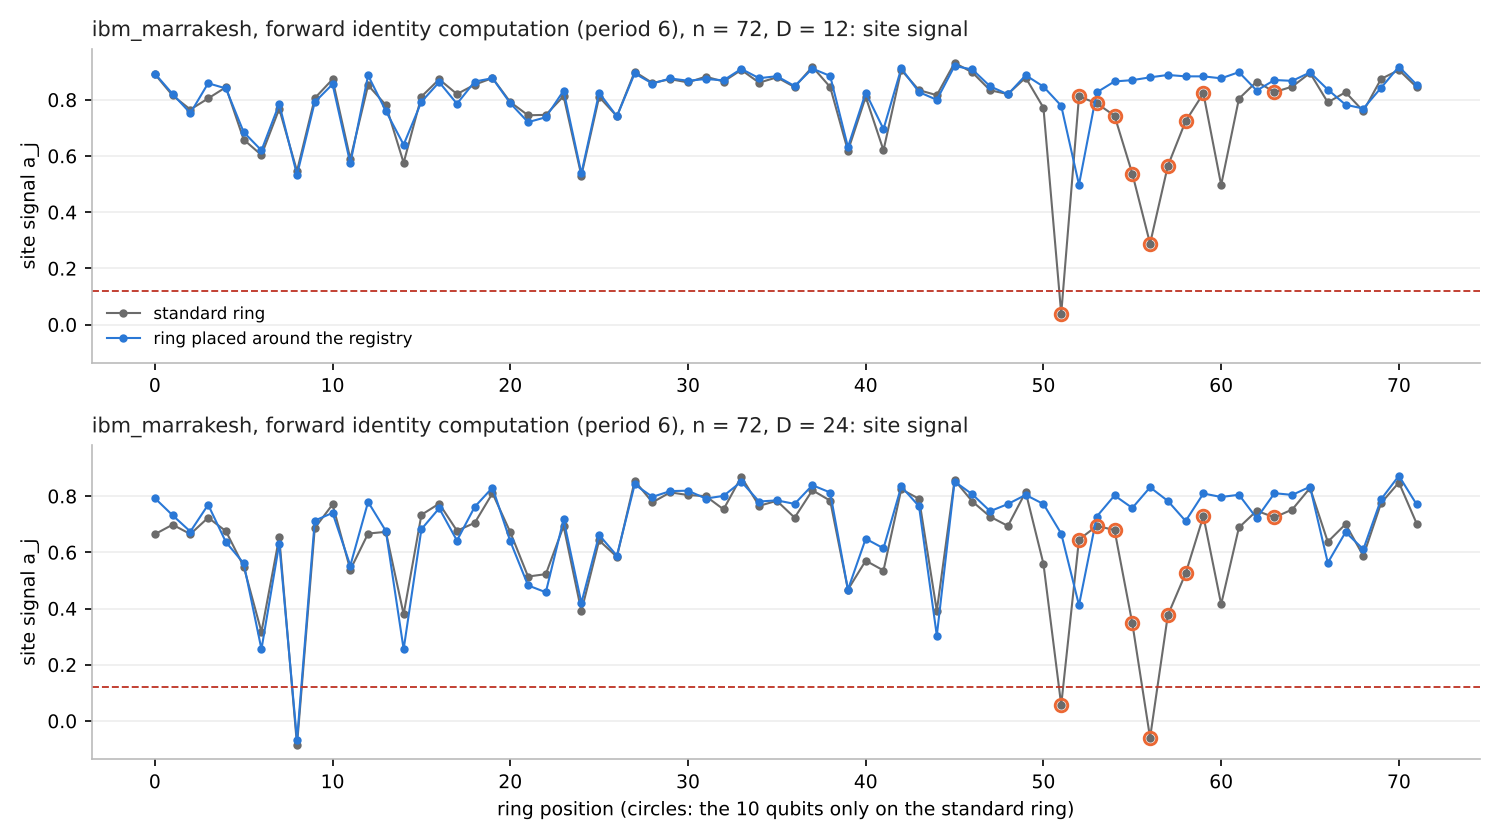
\includegraphics[width=\textwidth]{figures/self_check_m3b_sites.png}
\caption{Site signal of the forward computation, standard ring (grey) and avoiding ring (blue). Circles: the ten
qubits only on the standard ring.}
\label{fig:m3b}
\end{figure}

\begin{itemize}
\item \textbf{The show-off number and the essential one.} The show-off number is per-bit right 88.8\,\% $\to$
  90.8\,\%. The essential ones: the gain is 5\,\% and 8\,\% of the signal, and all of it sits in the ten swapped
  qubits (0.615 $\to$ 0.866 at $D=12$). On the 62 shared qubits the two rings read the same (0.802 against 0.808).
  % src: numbers.json m3b D12 per_bit (0.888, 0.908), swapped_mean (0.615, 0.866), common_mean (0.802, 0.808), n_common 62
\item \textbf{What kind of gain.} The listed path was weak that day, not dead, so nothing was unusable on the standard
  ring. The gain is accuracy, not width.
  % src: results/qca-m3b-2026-11-01/README.md ("The listed path today")
\item \textbf{The first attempt (kingston) did not reach its question.} It used $n$ layers of (H, CZ ring), the
  identity only after $D=n$ layers. At $n=40$ this meant 40 layers, beyond the readable depth of either ring: 0.009 on
  the standard ring and 0.020 on the avoiding one, under the declared floor of 0.05, so the result is INCONCLUSIVE.
  The $n=20$ control read 0.268. This was a design error. The lesson: a forward test needs a period shorter than $L^*$.
  % src: results/qca-m3-2026-11-01/README.md
\end{itemize}

\subsection{Repair: a local frame flip}\label{sec:repair}

\begin{itemize}
\item \textbf{The flip.} $X$ on chosen ring positions just before and after the CZ ring of every second layer, with a
  virtual $Z$ on the neighbours that need it. The ideal circuit is unchanged as an operator.
\item \textbf{Global against local.} A flip on all even positions lifted kingston's dead block but cost the healthy
  part of the ring. A flip around the block alone did nothing. Bisection then traced the gain to the first part of the
  run, and a flip on qubits 27 and 29 alone carried it.
  % src: results/black-stage2-2026-10-31/, results/black-stage3-2026-10-31/, results/black-bisect-2026-10-31/, results/black-fix-2026-10-31/ (README.md each)
\end{itemize}

\begin{table}[h]
\centering\small
\begin{tabular}{lccc}
\toprule
day & block, off $\to$ flip at 27, 29 ($D=24$) & difference & rest of the ring \\
\midrule
31 Oct & $-0.193 \to +0.129$ & $+0.322\pm0.007$ & $+0.008$ (NO COST) \\
1 Nov & $-0.185 \to +0.112$ & $+0.298\pm0.007$ & $+0.005$ (NO COST) \\
\bottomrule
\end{tabular}
% src: results/black-fix-2026-10-31/README.md (B3), results/fix-repeat-2026-11-01/README.md and ff_score.json (lfB3_D24)
\caption{The two-qubit flip on kingston's dead block (38, 49--55, 59). PERSISTS on the second day.}
\label{tab:repair}
\end{table}

\begin{figure}[h]
\centering
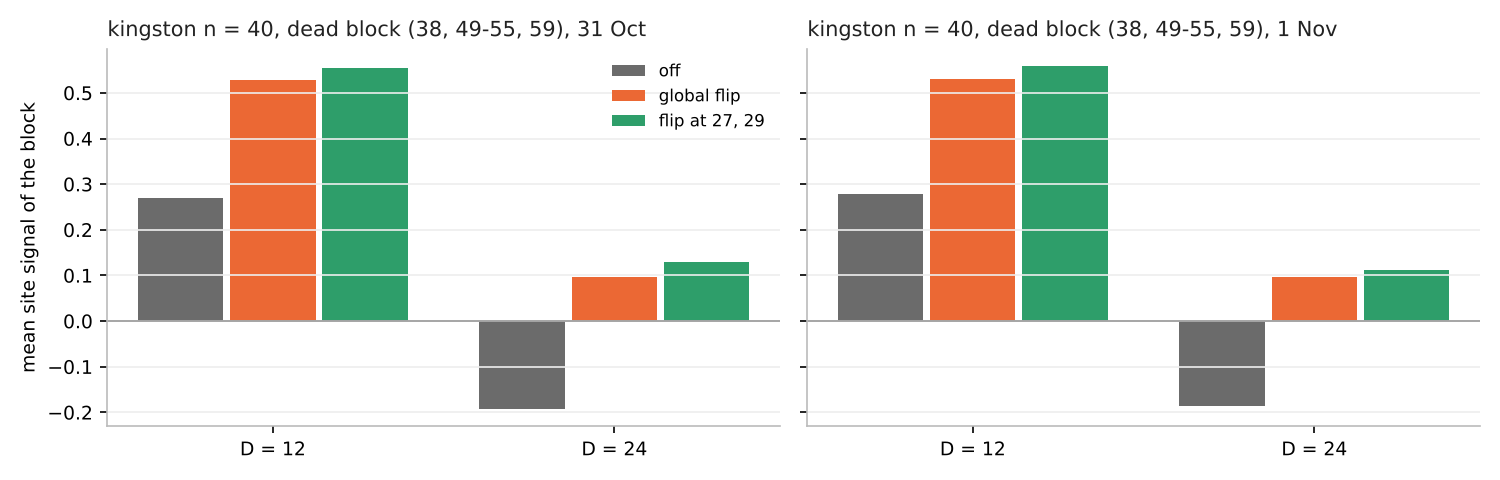
\includegraphics[width=\textwidth]{figures/self_check_repair.png}
\caption{Mean signal of kingston's dead block, flip off, global flip, and flip at 27 and 29, on two days.}
\label{fig:repair}
\end{figure}

\begin{itemize}
\item \textbf{Limits.} The block was not RECOVERED (0.8 $\times$ the rest). It reached about 0.30 $\times$ at $D=24$ and
  0.75 $\times$ at $D=12$. In usable sites the flip gave 22 $\to$ 25 at $D=24$ and 32 $\to$ 36 at $D=12$, against 40 of
  40 on the avoiding ring.
  % src: results/fix-repeat-2026-11-01/README.md (0.30 x, 0.75 x); numbers.json repair ("1 Nov D24 off" usable 22, "flip at 27, 29" 25; D12 32 -> 36)
\item \textbf{Mirror circuits only.} In simulation the flip cancels a static $ZZ$ error exactly only in a mirror
  circuit; for a forward computation it gives nothing, so the repair was not tried on one.
  % src: results/qca-m3-2026-11-01/sim/qca_fix.txt (n = 10, RZZ after every CZ touching the block, exact state
  % vectors: eps 0.1 off 0.923, local 0.939, global 0.920; eps 0.2 off 0.705, local 0.684, global 0.674)
\item \textbf{Conclusion.} Avoid first; repair only when the ring cannot avoid the path.
\end{itemize}

\subsection{Procedure failures, reported as results}\label{sec:failures}
\begin{itemize}
\item \textbf{Bisection stop rule.} The rule stopped on ``both halves HELP'', with $+0.019$ beside $+0.299$. Stop rules
  have weighed the size of effects since then.
  % src: results/black-bisect-2026-10-31/README.md
\item \textbf{Gray, stage 1.} Its precondition, the weak stretch, was absent when the test ran (Section~\ref{sec:what}),
  so nothing was judged.
\item \textbf{Forward test on kingston.} A design error (Section~\ref{sec:accuracy}).
\end{itemize}

\section{Discussion}
\begin{itemize}
\item \textbf{Width against accuracy.} Avoiding pays in width when a dead run lies on the standard ring (kingston
  $n=40$, 72; fez). It pays a little in accuracy when the path is only weak (marrakesh $n=72$). It changes nothing when
  the standard ring is clean (marrakesh $n=40$).
\item \textbf{What set the readable depth on these days.} With the placement held fixed: defects on the ring (on
  kingston $n=40$, Y2 $L^*$ 13--16 on the standard ring against 24 around the registry), the weight of what is read, a
  residual size effect of about two layers at $n\ge48$, and gray drift within hours. The order of the last three is not
  established.
\item \textbf{Why map-free matters here.} The calibration showed nothing at kingston's dead run \cite{paper5}. A layout
  scored by calibration error rates would not have avoided it.
\item \textbf{Psf-os.} The layers are being written as an open-source layer (AGPL-3.0) between a ring circuit and the
  device. Its skeleton reproduces the registry of the records byte for byte, and places the same rings as the test
  code. No performance of it is claimed here.
\end{itemize}

\section{Limitations}
\begin{itemize}
\item Three IBM heavy-hex devices, three days at most; one circuit family (the rule's ring); one forward computation,
  on one device and one day.
\item The registry's thresholds are fixed choices, not fitted; other choices would list other paths.
\item No error correction, no pulse access, and no cause of a defect is claimed.
\item At $n=72$ the avoiding ring did not reach the $n=20$ depth; we do not know why.
\item Repair works for mirror circuits only, and is weak at $D=24$.
\item Standard errors are shot noise only.
\end{itemize}

\section{Reproducibility}
{\sloppy
TOQB \cite{toqb}: \url{results/device-2026-10-30}, \url{results/device-2026-10-31-fez},
\url{results/coverage-days-2026-10-31-day1}, \url{results/coverage-days-2026-11-01-day2},
\url{results/clean-depth-2026-10-31}, \url{results/safe-ladder-2026-10-31}, \url{results/gray-stage1-2026-10-31},
\url{results/black-stage1-2026-10-31} to \url{results/black-fix-2026-10-31}, \url{results/fix-repeat-2026-11-01},
\url{results/two-devices-2026-11-01}, \url{results/qca-m3-2026-11-01}, \url{results/qca-m3b-2026-11-01},
\url{results/defect-list-replay-2026-10-31}; declarations in \url{prereg/}. The figures and every derived number
are made by \texttt{readable\_depth\_self\_check\_figures.py} from those records.\par}

\begin{table}[h]
\centering\small
\begin{tabular}{llll}
\toprule
test & declaration & SHA-256 (start) & fixed (CET) \\
\midrule
coverage days & \texttt{coverage\_days\_note.md} & 4941ddfa & 31 Oct 11:29 \\
clean depth & \texttt{clean\_depth\_note.md} & 2c45ee4b & 31 Oct 11:55 \\
safe ladder & \texttt{safe\_ladder\_note.md} & 67d10447 & 31 Oct 12:27 \\
gray stage 1 & \texttt{gray\_stage1\_note.md} & 25f6231a & 31 Oct 13:04 \\
black stage 1 & \texttt{black\_stage1\_note.md} & 04737044 & 31 Oct 13:22 \\
black stage 2 & \texttt{black\_stage2\_note.md} & 72aedffa & 31 Oct 13:41 \\
black stage 3 & \texttt{black\_stage3\_note.md} & 11f59455 & 31 Oct 13:58 \\
black bisection & \texttt{black\_bisect\_note.md} & 3697ce48 & 31 Oct 15:09 \\
black fix & \texttt{black\_fix\_note.md} & 0c72bbe8 & 31 Oct 15:30 \\
fix repeat & \texttt{fix\_repeat\_note.md} & 935d3a5d & 1 Nov 03:04 \\
two devices & \texttt{two\_devices\_note.md} & 91f2dbb8 & 1 Nov 11:30 \\
M3 (kingston) & \texttt{qca\_m3\_note.md} & 8a5618ca & 1 Nov 12:35 \\
M3, second form & \texttt{qca\_m3b\_note.md} & e3337f85 & 1 Nov 15:48 \\
coverage day 3 & \pending & & \\
\bottomrule
\end{tabular}
% src: the "Declaration" line of each results/<test>/README.md
\caption{Declarations, each fixed before the test's fetch.}
\label{tab:decl}
\end{table}

\appendix
\section{Calibration-only placement: a lower bound and a construction}\label{app:separation}

This appendix summarises a TOQB note~\cite{toqb} (\texttt{notes/separation\_2026-11-02/}, not declared). Its numbers
are simulations on a fake device, not device results.

\textbf{Lower bound.} Let $C(\theta)$ be the calibration numbers of a device state $\theta$: static per-element numbers
and the outcomes of \emph{isolated} experiments, in which no two couplers at distance one carry a two-qubit gate in
the same layer. A policy that reads only the coupling graph and $C$ gives the same placement law to all states with the
same $C$. Hence, for states $\theta_1,\dots,\theta_M$ with equal $C$, its worst expected regret is at least
$\frac1M\min_L\sum_k R_{\theta_k}(L)$ (the averaged two-point method of Le Cam~\cite{yu1997}). This is close to a
tautology. If a coupler $e$ carries an error only when a coupler at distance one is driven in the same layer, and a
ring through $e$ costs $\Delta$, the bound over all $e$ gives at least $n\Delta/|E_w|$ for a ring of $n$ qubits
($|E_w|=164$ working couplers on FakeKingston: $0.12\Delta$, $0.24\Delta$, $0.44\Delta$ at $n=20,40,72$).
The bound does not cover policies that read same-layer measurements (e.g.\ layer fidelity~\cite{mckay2023}), the
results of the user's own circuits, or their own tests of the day.
% src: TOQB notes/separation_2026-11-02/separation_note.tex, Lemma 1 and Corollary 1

\textbf{Upper bound, with its assumptions.} psf-os's scan reads each site from $4\times1000$ outcomes in $\{-1,+1\}$;
by Hoeffding's inequality~\cite{hoeffding1963} a site at distance $t$ from the line $0.12$ is misread with probability
at most $2e^{-2Nt^2}$ ($3\times10^{-13}$ one-sided at $t=0.12$, $N=1000$). This bounds the regret only if (A1) a dead
echo means a bad user circuit, (A2) the cost depends only on whether the ring holds a dead path, (A3) the comparator is
the rule's own placement with every dead path masked, not the best placement, and (A4) nothing changes between scan and
job. Near the line the bound says nothing: at $a_j=0.10$ it is $0.90$. The line $0.12$, the three sites and the two
jobs are chosen values.
% src: note Section 3, Proposition 1 and "What these numbers are not"

\textbf{Construction (Aer, FakeKingston, one planted coupler, no other noise).}

\begin{center}
\small
\begin{tabular}{lll}
\toprule
check & planted state & baseline \\
\midrule
the coupler alone ($m=2,8,32$) & counts identical to the baseline & 1.000 \\
with a neighbour in the same layer & 0.746, 0.269, 0.250 (Pauli) & 1.000 \\
Pauli $ZZ$ 0.15, scan at the Clifford point & usable 24 $\to$ 40 ($n=40$), 56 $\to$ 72 ($n=72$) & 40, 72 \\
coherent $R_{ZZ}(\pi/8)$, $n=20$, $h=0.6$ & usable 20 $\to$ 20, ring mean 0.40 $\to$ 1.00 & 1.000 \\
local frame flip (coherent) & every site 1.000 & 1.000 \\
\bottomrule
\end{tabular}
\end{center}
% src: TOQB notes/separation_2026-11-02/out/construction_result.json (rerun at home, identical except run time)

The error is invisible to the isolated benchmark and visible at once to a same-layer one, so it separates the two
kinds of policy. Two limits are part of the result. In the coherent model the planted stretch read $0.10$, just under
the line; it was read as dead in three of four readings of the same circuit and missed in one, so detection there is close to
chance. And the model's local flip repairs the stretch completely with no cost, while on \texttt{ibm\_kingston} the flip
at 27, 29 repaired the block only in part (Section~\ref{sec:results}); the device defect is consistent with this
construction but is not explained by a single static $ZZ$ term.

\section*{Acknowledgments}
We acknowledge the use of IBM Quantum services for this work. The views expressed are those of the authors, and do
not reflect the official policy or position of IBM or the IBM Quantum team. The device runs used the IBM Quantum
Open Plan, including its one-time promotion of 180 minutes of runtime.

\begin{thebibliography}{99}
\bibitem{paper5} TN Holdings, ``Readable Depth Without the Calibration Map: Formula Placement on Heavy-Hex Devices,
and a Defect the Calibration Does Not Show'', version 1.1 (2026), doi:10.5281/zenodo.23827536.
\bibitem{paper4} TN Holdings, ``Folding a Ring onto Heavy-Hex: Formula-Built Schedules with Provable Gate Counts, and
What Their Signal Shows on Twins and Devices'', version 1.3 (2026), doi:10.5281/zenodo.23826764.
\bibitem{paper3} TN Holdings, ``When a Quantum Compiler Looks Like a Better Learner: Confounds in Quantum Machine
Learning Comparisons'', version 1.3 (2026), doi:10.5281/zenodo.23826596.
\bibitem{toqb} TN Holdings, TOQB, the test bench for PSF-Zero's training and device runs (2026).
\bibitem{proctor2022} T. Proctor, K. Rudinger, K. Young, E. Nielsen and R. Blume-Kohout, ``Measuring the capabilities
of quantum computers'', Nature Physics (2022); arXiv:2008.11294.
\bibitem{mckay2023} D. C. McKay, I. Hincks, E. J. Pritchett, M. Carroll, L. C. G. Govia et al., ``Benchmarking
Quantum Processor Performance at Scale'', arXiv:2311.05933 (2023).
\bibitem{vf2post} Qiskit documentation, \texttt{qiskit.transpiler.passes.VF2PostLayout},
\url{https://quantum.cloud.ibm.com/docs/api/qiskit/qiskit.transpiler.passes.VF2PostLayout}.
\bibitem{klimov2018} P. V. Klimov et al., ``Fluctuations of energy-relaxation times in superconducting qubits'',
Phys. Rev. Lett. 121, 090502 (2018); arXiv:1809.01043.
\bibitem{wallman2016} J. J. Wallman and J. Emerson, ``Noise tailoring for scalable quantum computation via randomized
compiling'', Phys. Rev. A 94, 052325 (2016).
\bibitem{yu1997} B. Yu, ``Assouad, Fano, and Le Cam'', in \emph{Festschrift for Lucien Le Cam}, Springer, New York (1997),
doi:10.1007/978-1-4612-1880-7\_29.
\bibitem{hoeffding1963} W. Hoeffding, ``Probability inequalities for sums of bounded random variables'',
J. Amer. Statist. Assoc. \textbf{58}(301), 13--30 (1963).
\end{thebibliography}

\end{document}
